\section{Bakti QIlan Mufid | 1174083}
\subsection{Soal 1}
Apa itu fungsi device manager di windows dan folder /dev di linux.
\begin{itemize}
	\item Device Manager: Device Manager dalam komputer windows, adalah perluasan dari Microsoft Management Console. Device Manager menampilkan seluruh hardware yang bisa di-inisialisasi (dikenali) oleh Windows. dan fungsi dari Device Manager ini ialah dalam mengelola (manage) semua hardware yang terpasang (dan terdeteksi)dalam suatu sistem Windows. Hardware seperti harddisk, kartu VGA, sound, keyboard, perangkat USB dll. akan sangat mudah untuk dikonfigurasi dari dalam Device Manager ini. Device Manager paling sering digunakan untuk pengelolaan driver suatu hardware. Misalnya instalasi driver, uninstal driver, update driver, rollback driver, dan bermacam problem yang berkaitan dengan driver suatu hardware.
	\item folder /dev berisi semua drive harddisk atau hardware seperti modem, CD/DVD/Blu-ray dsb. Hanya saja disini hanya merupakan link dan bukan isi, contohnya hdd partisi 1 ada di /dev/sda1 dan DVD-rom ada di /dev/sr0. untuk melihat isinya, harus dilakukan mounting (mount) terlebih dahulu.
\end{itemize}

\subsection{Soal 2}

Jelaskan langkah-langkah instalasi driver dari arduino UNO di Windows

Berikut ini adalah langkah-langkah instalasi driver dari arduino UNO di Windows
	\begin{itemize}
		\item Pertama pastikan Arduino IDE telah terinstall.
		\item Hubungkan port USB Arduino Uno ke port USB PC.
			\begin{figure}[ht]
				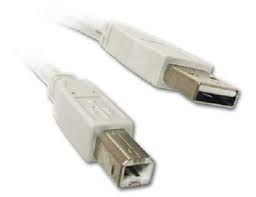
\includegraphics[width=10cm]{figures/5/1174083/Teori/kabel.jpg}
				\centering
				\caption{menghubungkan port.}
			\end{figure}
		\item Lalu pada bagian kanan didesktop PC anda, akan muncul popup “Installing device driver software” seperti pada gambar dibawah ini.
			\begin{figure}[ht]
				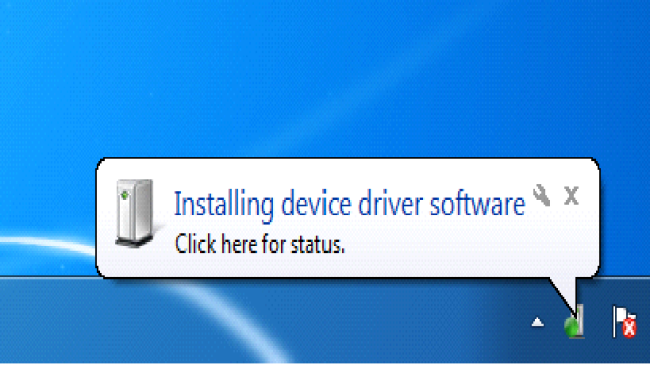
\includegraphics[width=10cm]{figures/5/1174083/Teori/2.png}
				\centering
				\caption{muncul pop up.}
			\end{figure}
		\item SIstem operasi Windows tidak menyediakan driver untuk Arduino Uno seperti yang terlihat pada gambar dibawah ini, lalu proses instalasinya harus dilakukan secara manual.
			\begin{figure}[ht]
				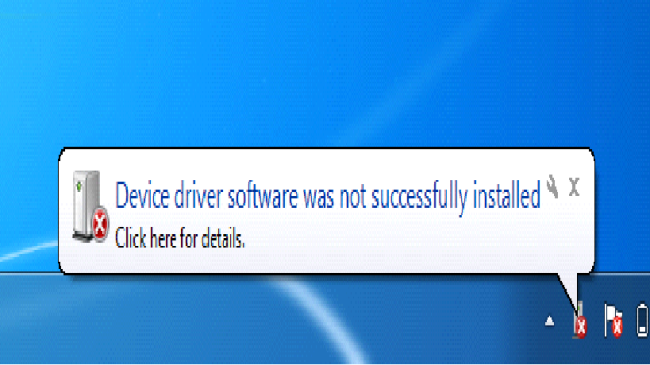
\includegraphics[width=10cm]{figures/5/1174083/Teori/3.png}
				\centering
				\caption{instalasi manual.}
			\end{figure}
		\item Buka Device Manager, caranya pada bagian Search Program and Files lalu ketikkan “device manager” (tanpa tanda petik), perhatikan gambar dibawah ini. Pada bagian Control Panel akan muncul Device Manager, klik untuk menjalankan.
			\begin{figure}[ht]
				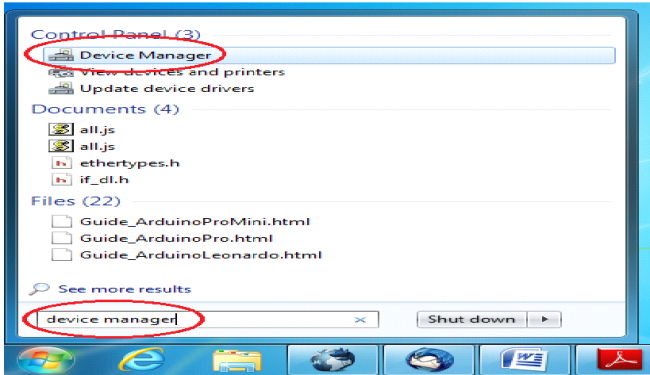
\includegraphics[width=10cm]{figures/5/1174083/Teori/4.png}
				\centering
				\caption{membuka device manager.}
			\end{figure}
		\item Cari Unknown device pada bagian Other device, biasanya terdapat tanda seru berwarna kuning, itu disebabkan karena penginstallan tidak berjalan dengan sempurna.
			\begin{figure}[ht]
				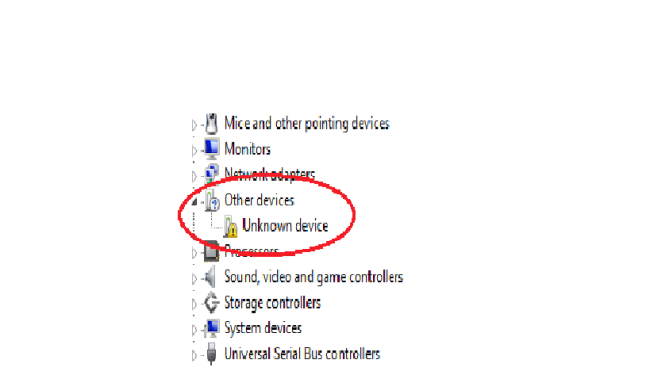
\includegraphics[width=10cm]{figures/5/1174083/Teori/5.png}
				\centering
				\caption{tanda seru.}
			\end{figure}
		\item Klik kanan pada “Unknown device” kemudian pilih Update Driver Software.		
			\begin{figure}[ht]
				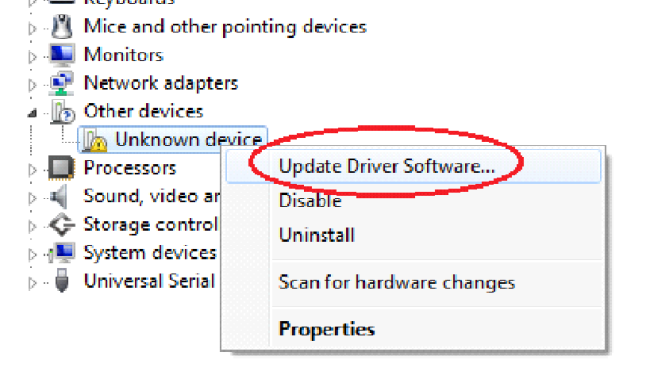
\includegraphics[width=10cm]{figures/5/1174083/Teori/6.png}
				\centering
				\caption{update Driver Software.}
			\end{figure}
		\item Pilih Browse my computer for driver software.
			\begin{figure}[ht]
				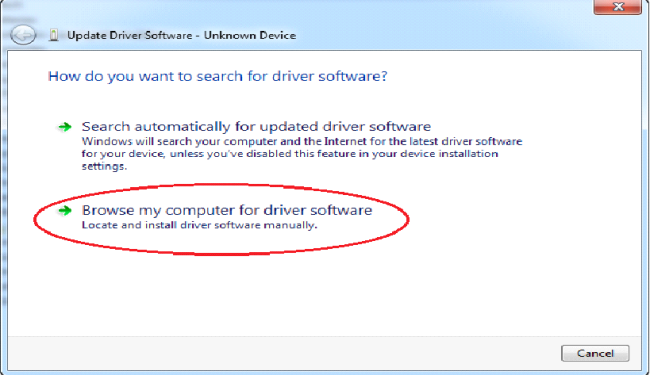
\includegraphics[width=10cm]{figures/5/1174083/Teori/7.png}
				\centering
				\caption{Browse my computer.}
			\end{figure}
		\item Arahkan lokasi folder ke folder \verb|..\arduino-1.0.5\drivers.| Pastikan check-box lalu centang include subfolders. Klik Next untuk melanjutkan instalasi driver.
			\begin{figure}[ht]
				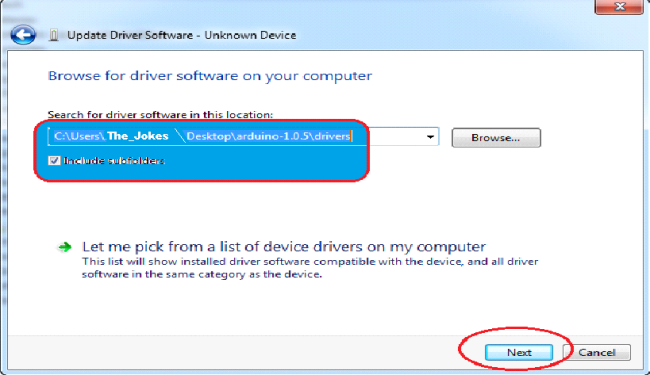
\includegraphics[width=10cm]{figures/5/1174083/Teori/8.png}
				\centering
				\caption{mengarahkan lokasi ke folder.}
			\end{figure}
		\item Kemudian lanjutkan dengan mengklik Install pada tampilan Windows Security.
			\begin{figure}[ht]
				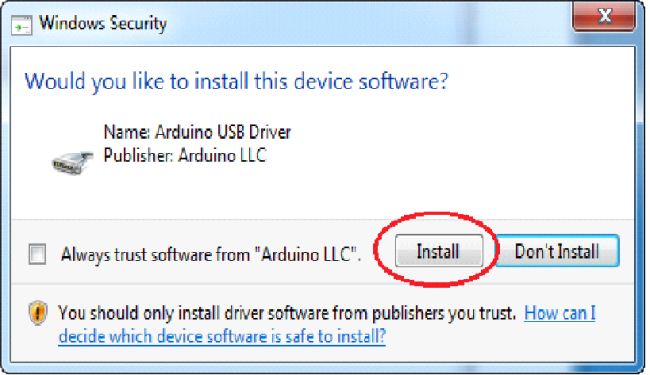
\includegraphics[width=10cm]{figures/5/1174083/Teori/9.png}
				\centering
				\caption{Klik Install.}
			\end{figure}
		\item Jika instalasi driver berhasil maka akan muncul Windows has successfully updated your driver software.
			\begin{figure}[ht]
				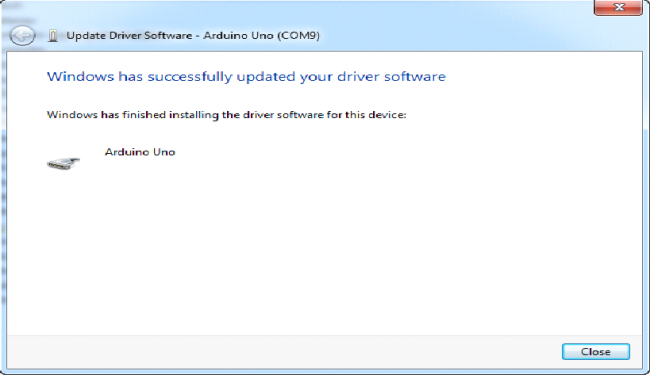
\includegraphics[width=10cm]{figures/5/1174083/Teori/10.png}
				\centering
				\caption{Successfully}
			\end{figure}
		\item Perhatikan dan ingat nama COM Arduino Uno, karena nama COM ini yang akan digunakan untuk meng-upload program nantinya.
			\begin{figure}[ht]
				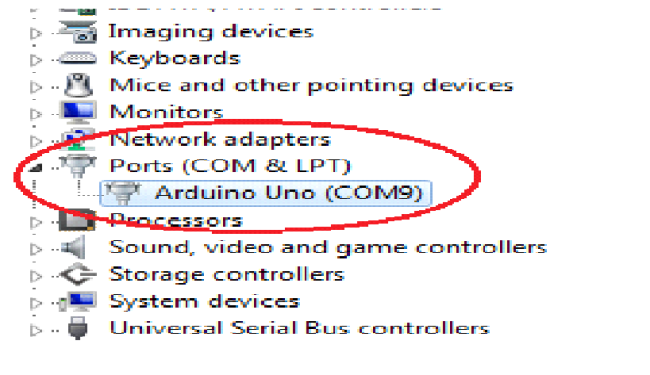
\includegraphics[width=10cm]{figures/5/1174083/Teori/11.png}
				\centering
				\caption{Selesai.}
			\end{figure}
	\end{itemize}
	
\subsection{Soal 3}
Jelaskan bagaimana cara membaca baudrate dan port dari komputer yang sudah
terinstall driver

Untuk melihat atau membaca baudrate dan port kita hanya perlu menginstall Arduino IDE, setelah itu buka menu serial monitor yang berada di tab tools. Dari sana akan terlihat baik baudrate dan port yang sedang digunakan oleh arduino anda.

\subsection{Soal 4}
Jelaskan sejarah library pyserial

PySerial merupakan sebuah library yang digunakan untuk komunikasi ke port serial terutama untuk mikrokontroller. PySerial pertama kali diluncurkan pada tahun 2002 yang makin berkembang dalam setiap versinya hingga tahun 2017 lalu.

\subsection{Soal 5}
Jelaskan fungsi-fungsi apa saja yang dipakai dari library pyserial

Fungsi-fungsi yang dipakai dari library PySerial, yaitu:
\begin{enumerate}
	\item Serial - fungsi ini untuk membuka port serial.
	\item read(size) - fungsi ini untuk membaca jumlah byte dari port serial.
	\item write(data) - fungsi ini menulis data lewat port serial.
	\item readline() - fungsi ini membaca sebuah string dari port serial.
	\item close() - fungsi ini untuk menutup port serial.
\end{enumerate}

\subsection{Soal 6}
Jelaskan kenapa butuh perulangan dan tidak butuh perulangan dalam membaca serial

Karena dalam pembacaan serial dalam arduino yang memerlukan membaca data secara berulang-ulang harus dengan perulangan. dan tidak butuh perulangan ketika membaca data hanya dilakukan sekali saja.

\subsection{Soal 7}
Jelaskan bagaimana cara membuat fungsi yang mengunakan pyserial

tata cara untuk membuat pyserial seperti pada kode dibawah

\lstinputlisting[firstline=10, lastline=16]{src/5/1174083/Teori/1174083.py}


\subsection{Cek Plagiat}
\begin{figure}[H]
	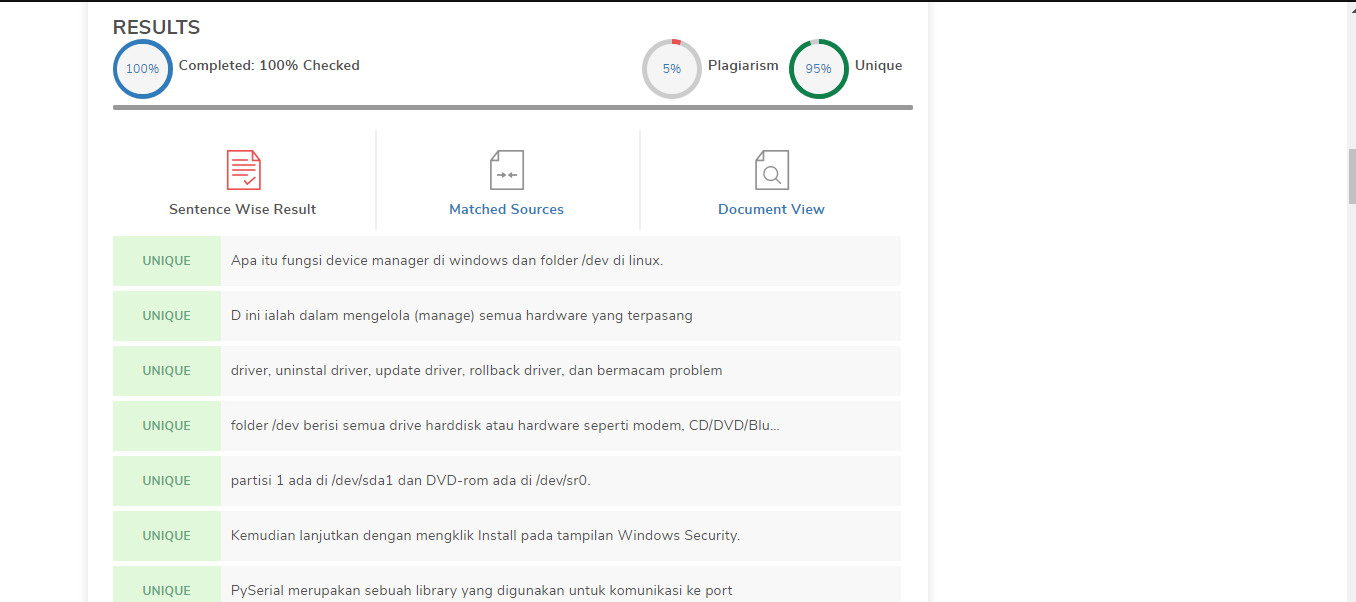
\includegraphics[width=10cm]{figures/5/1174083/Teori/plagiat1.png}
	\centering
	\caption{Hasil cek plagiarism.}
\end{figure}

\subsection{Kode Program}
\begin{figure}[ht]
	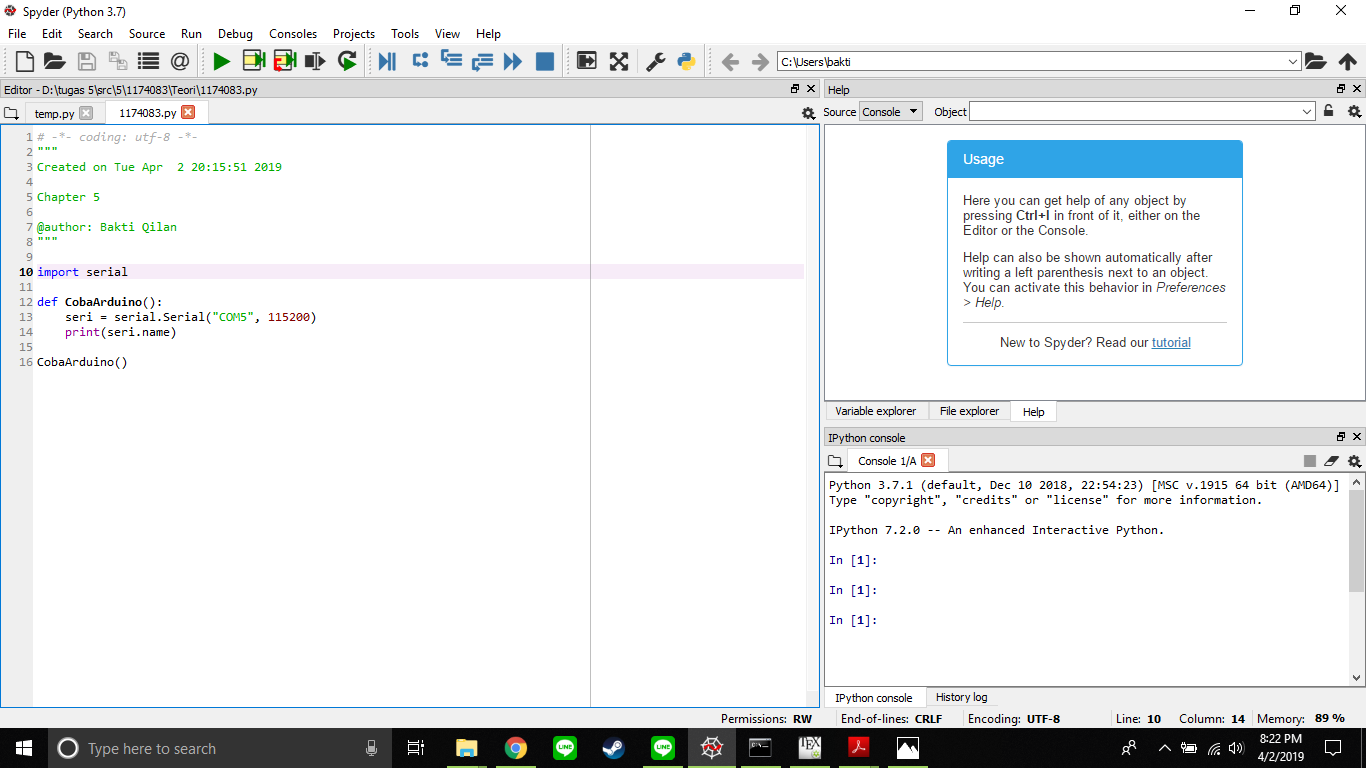
\includegraphics[width=10cm]{figures/5/1174083/Teori/kodefungsi.png}
	\centering
	\caption{Kode program fungsi.}
\end{figure}

%%%%%%%%%%%%%%%%%%%%%%%%%%%%%%%%%%%%%%%%%%%%%%%%%%%%%%%%%%%%%%%%%%%%%%%%%%%%%%%%%%%%%%%%%%%%%%%%%%%%%%%%%
\section{Mochamad Arifqi Ramadhan | 1174074}
\subsection{Soal 1}

\textbf{Fungsi Device manager di Windows & Folder /dev di Linux}
\begin{itemize}
\item Fungsi Device Manager di Windows
	Device Manager akan sangat membantu dalam mengelola (manage) semua hardware yang terpasang (dan terdeteksi) dalam suatu sistem Windows. Hardware seperti harddisk, kartu VGA, sound, keyboard, perangkat USB dll. akan sangat mudah untuk dikonfigurasi dari dalam Device Manager ini. ( mengetahui port arduinno)

\item Fungsi Folder /dev di Linux
/dev berfungsi mengetahui  direktori yang tersimpan konfigurasi device/hardware pada sistem. Contohnya folder /dev artinya file-file tersebut berada.

	
\subsection{Soal 2}	
\textbf{Intall Arduino}

Cara instalasi driver arduino :
		\begin{enumerate}
			\item Pertama download software arduino, extract bila file zip/rar
			\item hubungkan Port USB Arduino UNO ke Port USB PC
			\item lalu windows akan memunculkan pop up yang memberitahu bahwa ingin menginstall dirver, tapi nanti tidak akan menemukan drivernya
			\item buka Device Manager, setelah Device Manager terbuka, silahkan cari “Unknown Device” yang berada di Other Device.
			\item klik kanan pada unknown device tersebut lalu pilih update driver software
			\item pilih browse my computer for driver software lalu masukkan directory dimana anda menyimpan driver arduino yang telah anda download tadi
			\item setelah itu klik install dan tunggu hingga proses selesai
			\item arduino pun sudah terbaca di pc anda 
		\end{enumerate}


\subsection{Soal 3}

\textbf{Membaca baudrate dan port di komputer}
Untuk membaca baudrate dan port di komputer pertama hbungkan arduino dengan komputer
1. bisa dengan cara membuka Device manager
2. lalu pilih ports (COM  dan LPT)
3. pilih COM yang terhubung
4. Pilih port setting dan lihat di Bit per second untuk baudrate

Sedangkan untuk port
lakukan proses 1 dan 2 seperti diatas
Dan port dari arduino telah terbaca oleh PC
	
\subsection{Soal 4}

\textbf{Sejarah library PySerial}

	PySerial adalah library yang menyediakan dukungan untuk koneksi serial ("RS-232") melalui berbagai perangkat yang berbeda: port serial gaya lama, dongle Bluetooth, port infra merah, dan sebagainya. Ini juga mendukung port serial jarak jauh melalui RFC 2217 (sejak V2.5). dan PySerial pertama kali diluncurkan pada tahun 2002 yang makin berkembang dalam setiap versinya hingga tahun 2017 lalu.

\subsection{Soal 5}

\textbf{Fungsi-Fungsi di library PySerial}
\begin{itemize}
\item print(ser.name)         - meriksa port yang benar-benar digunakan
\item ser.write(b'hello')     	- menulis tipe data string
\item ser.readline()  	- untuk membaca string dari port serial
\item  ser.read()         	 - membaca satu port
\item ser.close()         	- menutup port
\end{itemize}

\subsection{Soal 6}

\textbf{Perulangan dan Tidak Perulangan}
	Perulangan digunakan untuk melakukan scanning/pengambilan data secara terus menerus(continue) artinya pengeksekusiannya terus berjalan auto selama ada scanning/pengambilan data. Sedangkan Tidak Pengulangan digunakan untuk menscanning/pengambilan data secara real time atau pengambilan datanya hanya sekali saja.


\subsection{Soal 7}

\textbf{Membuat fungsi dengan PySerial}


 Import Serial

Ser = serial.Serial (port, baudrate) #membuka serial port
Ketengan : Ser adalah objek Serial, serial adalah kelas, Serial adalah method

contoh fungsi : data = Ser.readline() artinya membaca data


\subsection{Bukti Screenshoot}

\begin{figure}[H]
	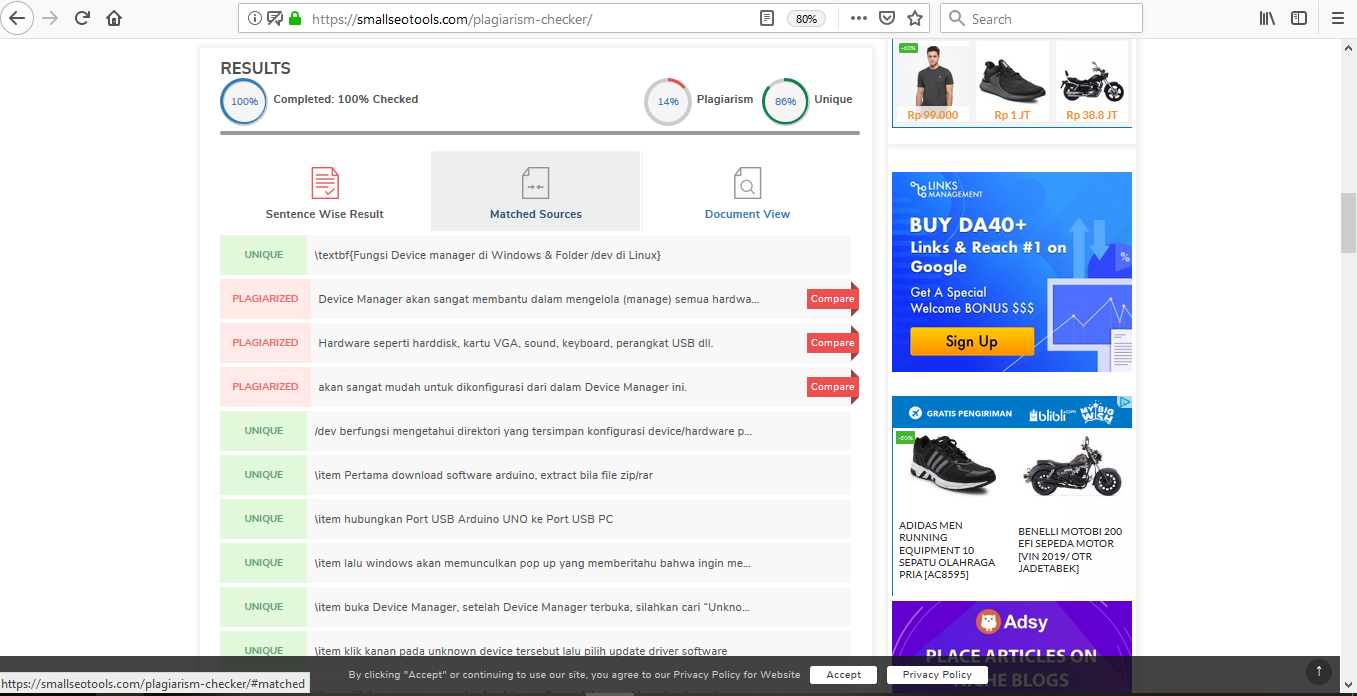
\includegraphics[width=10cm]{figures/5/1174074/Teori/plagiarisme2.png}
	\centering	
	\caption{Cek Plagiat}
\end{figure}
%%%%%%%%%%%%%%%%%%%%%%%%%%%%%%%%%%%%%%%%%%%%%%%%%%%%%%%%%%%%%%%%%%%%%%%%%%%%%%%%%%%%%%%%%%%%%%%%%%%%%%%%%%%%%%%%%%%%